% !TeX program = xelatex
% UTF-8. Compile twice with XeLaTeX.
\documentclass[UTF8,a4paper,zihao=5,fontset=none]{ctexart}
\usepackage[left=23mm,right=23mm,top=20mm,bottom=21mm,footskip=10mm]{geometry}
\usepackage{fontspec}
\setmainfont{Times New Roman}
\setsansfont{Times New Roman}
\setmonofont{Consolas}[Scale=0.91]
\newfontfamily{\circledfont}{Segoe UI Symbol}
\setCJKmainfont{SimSun}[AutoFakeBold=2]
\setCJKsansfont{SimHei}
\setCJKmonofont{SimSun}
\setCJKfamilyfont{hei}{SimHei}
\newcommand{\heiti}{\CJKfamily{hei}}
\usepackage{amsmath,amssymb,array,booktabs,longtable,tabularx,makecell}
\usepackage{graphicx,tikz,circuitikz,caption,listings,needspace}
\usetikzlibrary{arrows.meta,positioning,calc}
\usepackage[hidelinks,unicode,pdfencoding=auto]{hyperref}
\hypersetup{pdftitle={作业2 STM32与Cortex-M4体系结构},pdfauthor={彭俊杰},pdfsubject={嵌入式系统课程作业}}
\ctexset{
  section={format=\heiti\fontsize{11.5}{16.5}\selectfont,number=\arabic{section}.,aftername=\hspace{0.4em},beforeskip=11pt,afterskip=8pt},
  subsection={format=\heiti\fontsize{11}{16}\selectfont,number={{\circledfont\ifcase\value{subsection}\or①\or②\or③\or④\fi}},aftername=\hspace{0.4em},beforeskip=10pt,afterskip=7pt}
}
\pdfstringdefDisableCommands{\def\circledfont{}}
\linespread{1.22}
\setlength{\parindent}{2em}
\setlength{\parskip}{3pt}
\setlength{\emergencystretch}{1.5em}
\raggedbottom
\pagestyle{plain}
\clubpenalty=10000
\widowpenalty=10000
\displaywidowpenalty=10000
\captionsetup{font=small,labelsep=quad,justification=centering,singlelinecheck=false,hypcap=false,skip=6pt}
\captionsetup[table]{position=top,skip=5pt}
\newcolumntype{L}[1]{>{\raggedright\arraybackslash}m{#1}}
\newcolumntype{C}[1]{>{\centering\arraybackslash}m{#1}}
\newcolumntype{Y}{>{\raggedright\arraybackslash}X}
\newcolumntype{Z}{>{\centering\arraybackslash}X}
\renewcommand{\tabularxcolumn}[1]{m{#1}}
\newcommand{\TableHead}[1]{\multicolumn{1}{c}{\heiti #1}}
\newcommand{\hex}[1]{\texttt{0x#1}}
\newcommand{\code}[1]{\texttt{#1}}
\newcommand{\shortcell}[1]{{\centering #1\par}}
\newcommand{\question}[1]{\begingroup\linespread{1}\fontsize{10.5}{15.5}\selectfont\noindent\textbf{题目}\quad #1\par\endgroup\vspace{4pt}}
\newenvironment{datatab}{\par\begingroup\centering\linespread{1}\fontsize{10.5}{14.5}\selectfont\setlength{\tabcolsep}{5pt}\renewcommand{\arraystretch}{1.14}\setlength{\extrarowheight}{2pt}}{\par\endgroup\vspace{5pt}}
\tikzset{
  block/.style={draw=black!70,fill=black!3,line width=0.55pt,align=center,inner sep=5pt,font=\linespread{1}\fontsize{10.5}{14.5}\selectfont},
  arrow/.style={-{Stealth[length=2mm]},line width=0.7pt},
  wire/.style={line width=0.65pt}
}
\lstdefinestyle{cstyle}{
  language=C,basicstyle=\linespread{1}\ttfamily\fontsize{9.4}{11.7}\selectfont,
  keywordstyle=\bfseries,commentstyle=\normalfont\itshape,
  stringstyle=\ttfamily,numbers=left,numberstyle=\ttfamily\fontsize{7.5}{10}\selectfont,
  numbersep=8pt,xleftmargin=19pt,xrightmargin=1pt,
  showstringspaces=false,tabsize=4,keepspaces=true,columns=fullflexible,
  breaklines=true,breakatwhitespace=true,aboveskip=5pt,belowskip=7pt,
  frame=none,captionpos=t
}
\lstset{style=cstyle}

\begin{document}
\begin{center}
  {\heiti\fontsize{22}{28}\selectfont 作业2\par}
  \vspace{3pt}
  {\heiti\fontsize{13}{18}\selectfont STM32与Cortex-M4体系结构\par}
  \vspace{5pt}
  {\fontsize{11}{16}\selectfont 彭俊杰\qquad 智装备241\qquad 2024306100324\par}
\end{center}
\vspace{-3pt}

\section{说明下列英文缩写的含义：ARM、AHB、AHB-Lite、APB、PPB、DAP（JTAG、SWD）、MPU、FPU、NVIC、ISR、Bitband、SCS、SysTick、MSP、PC、SP、GPIO、TIM、UART、CANBUS。}

\begingroup
\linespread{1}
\fontsize{9.7}{13.1}\selectfont
\setlength{\tabcolsep}{4pt}
\renewcommand{\arraystretch}{1.05}
\setlength{\extrarowheight}{1.8pt}
\setlength{\LTpre}{2pt}
\setlength{\LTpost}{0pt}
\begin{longtable}{@{}C{17mm}C{43mm}L{97mm}@{}}
\caption{英文缩写与含义}\\
\toprule
\TableHead{缩写} & \TableHead{英文名称} & \TableHead{含义}\\
\midrule
\endfirsthead
\toprule
\TableHead{缩写} & \TableHead{英文名称} & \TableHead{含义}\\
\midrule
\endhead
\bottomrule
\endfoot
ARM & Advanced RISC Machines & 处理器架构及处理器 IP 的名称，采用精简指令集设计。\\
AHB & Advanced High-performance Bus & AMBA 高性能总线，连接处理器、存储器及高速外设。\\
AHB-Lite & Advanced High-performance Bus Lite & 单主设备 AHB 简化协议；多层矩阵可连接多个主端口。\\
APB & Advanced Peripheral Bus & 面向低带宽外设的简单总线，经桥与 AHB 相连。\\
PPB & Private Peripheral Bus & 内核私有外设总线，访问系统控制、调试等部件。\\
DAP & Debug Access Port & 调试访问端口，由调试端口和访问端口组成。\\
JTAG & Joint Test Action Group & IEEE 1149.1 边界扫描接口，亦用于处理器调试。\\
SWD & Serial Wire Debug & 串行线调试接口，主要信号为 SWDIO 和 SWCLK。\\
MPU & Memory Protection Unit & 存储器保护单元，按区域设置访问权限和存储属性。\\
FPU & Floating-Point Unit & 浮点运算单元；F407 与 L496 集成单精度 FPU。\\
NVIC & Nested Vectored Interrupt Controller & 嵌套向量中断控制器，管理中断使能、挂起和优先级。\\
ISR & Interrupt Service Routine & 中断服务程序，响应中断时执行的处理函数。\\
Bitband & Bit-banding & 位带机制：别名区的一个 32 位字映射原区域的一位。\\
SCS & System Control Space & 系统控制空间，包含 SCB、NVIC、SysTick 寄存器。\\
SysTick & System Tick Timer & 内核 24 位递减定时器，常用于系统节拍和延时。\\
MSP & Main Stack Pointer & 主栈指针；复位后使用，异常处理模式固定使用。\\
PC & Program Counter & 程序计数器 R15，保存程序执行地址。\\
SP & Stack Pointer & 栈指针 R13；线程模式可选择 MSP 或 PSP。\\
GPIO & General-Purpose Input/Output & 通用输入输出，引脚可配置为输入、输出或复用功能。\\
TIM & Timer & 定时器，支持定时计数、输入捕获、输出比较和 PWM。\\
UART & Universal Asynchronous Receiver/Transmitter & 通用异步收发器；USART 还支持同步通信。\\
CANBUS & Controller Area Network Bus & 控制器局域网总线，采用基于标识符的非破坏性逐位仲裁。\\
\end{longtable}
\endgroup

\clearpage
\section{简要画图说明 ARM Cortex-M4 对存储器映射如何划分地址区域的，（自学）标出 GPIO、SysTick、CAN 这些外设寄存器所在的地址在哪个区域？}

Cortex-M4 采用 32 位字节地址，地址范围为 \hex{00000000}～\hex{FFFFFFFF}，共 $2^{32}$ 字节，即 4 GiB。

\begin{figure}[!ht]
\centering
\begin{tikzpicture}[x=1cm,y=1cm]
  \draw[arrow] (0,0.25)--(0,6.5);
  \node[align=center,font=\small] at (0,6.9) {高地址};
  \node[align=center,font=\small] at (0,-0.15) {低地址};
  \foreach \i/\name/\lo/\hi/\size in {
    0/系统区/E0000000/FFFFFFFF/512 MiB,
    1/外部设备区/A0000000/DFFFFFFF/1 GiB,
    2/外部 RAM 区/60000000/9FFFFFFF/1 GiB,
    3/外设区/40000000/5FFFFFFF/512 MiB,
    4/SRAM 区/20000000/3FFFFFFF/512 MiB,
    5/代码区/00000000/1FFFFFFF/512 MiB}{
      \pgfmathsetmacro{\yc}{5.95-1.07*\i}
      \draw[fill=black!3,draw=black!60] (0.65,\yc-0.48) rectangle (14.7,\yc+0.48);
      \node[align=center,text width=3.0cm,font=\linespread{1}\fontsize{10}{12}\selectfont] at (2.3,\yc) {\name\ifnum\i=0\\SysTick\fi\ifnum\i=3\\GPIO / CAN\fi};
      \node[align=center,font=\ttfamily\fontsize{10}{14}\selectfont] at (7.5,\yc) {0x\lo\enspace--\enspace0x\hi};
      \node[align=center,text width=2.0cm,font=\small] at (13.4,\yc) {\size};
  }
\end{tikzpicture}
\caption{Cortex-M4 地址空间分区}
\label{fig:memory}
\end{figure}

\begin{datatab}
\captionof{table}{STM32F407 外设地址与所属区域}
\begin{tabularx}{\linewidth}{@{}C{21mm}C{35mm}C{28mm}Z@{}}
\toprule
\TableHead{模块} & \TableHead{基址} & \TableHead{区域} & \TableHead{挂接位置}\\
\midrule
GPIOA & \hex{40020000} & 外设区 & AHB1\\
GPIOF & \hex{40021400} & 外设区 & AHB1\\
CAN1 & \hex{40006400} & 外设区 & APB1\\
CAN2 & \hex{40006800} & 外设区 & APB1\\
SysTick & \hex{E000E010} & 系统区 & PPB 中的 SCS\\
\bottomrule
\end{tabularx}
\end{datatab}

从总线归属分析：GPIOA 与 GPIOF 挂接在 AHB1 高速外设总线上，CAN 挂接在 APB1 总线上；而 SysTick 属于内核私有外设，直接映射于系统控制空间（SCS，\hex{E000E000}～\hex{E000EFFF}），经由私有外设总线（PPB，\hex{E0000000}～\hex{E00FFFFF}）访问，不占用外设总线带宽。SysTick 的 CTRL、LOAD、VAL、CALIB 寄存器地址依次为 \hex{E000E010}、\hex{E000E014}、\hex{E000E018} 与 \hex{E000E01C}。此外，Cortex-M4 在 SRAM 区与外设区底部 1 MB 空间分别支持位带别名区映射，便于实现原子位操作。

\clearpage
\section{画简图说明有关中断的概念（罗列关键词），并说明 ARM Cortex-M4 微处理器异常/中断向量表的作用是什么？}

Cortex-M4 采用统一的异常管理模型，将内核服务故障与外部中断统筹管理。外设通过 IRQ 线向 NVIC 提交请求，SysTick、SVC、PendSV 则属于内核异常。中断从请求到响应的硬件处理时序见图 \ref{fig:interrupt}。

\begin{figure}[!ht]
\centering
\begin{tikzpicture}
  \node[block,text width=2.7cm,minimum height=2.0cm] (src) at (1.7,0) {外设中断源\\[4pt]EXTI / TIM / CAN\\产生 IRQ};
  \node[block,text width=3.8cm,minimum height=4.3cm] (nvic) at (6.8,0) {\textbf{NVIC}\\[8pt]使能与屏蔽\\[5pt]挂起 Pending\\[5pt]优先级仲裁\\[5pt]抢占与嵌套};
  \node[block,text width=3.9cm,minimum height=4.3cm] (cpu) at (12.2,0) {\textbf{Cortex-M4 内核}\\[8pt]自动压栈\\[5pt]读取向量\\[5pt]执行 ISR\\激活 Active\\[5pt]异常返回与恢复现场};
  \draw[arrow] (src.east)--(nvic.west);
  \draw[arrow] (nvic.east)--(cpu.west);
\end{tikzpicture}
\caption{中断响应过程及关键词}
\label{fig:interrupt}
\end{figure}

当中断请求满足使能与优先级仲裁条件时，处理器硬件自动在当前堆栈压入基础栈帧（R0～R3、R12、LR、PC 与 xPSR），并由硬件直接从向量表装载 ISR 入口执行。异常返回时，特定的 EXC\_RETURN 编码触发硬件自动出栈并恢复现场。编写 ISR 时，须按外设规则显式清除中断挂起标志，防止异常返回后发生错误重入。

异常状态包含未激活、挂起（已记录请求）、激活（正在执行服务）及激活并挂起。可配置优先级的数值越小代表优先级越高；抢占优先级支持高优先级中断打断低优先级执行形成嵌套，子优先级则在抢占优先级相同时决定排队次序。

\subsection*{向量表的作用}
向量表将异常编号与处理函数入口对应起来，每项占 4 字节。第 0 项保存初始 MSP，第 1 项保存复位入口；其余表项保存异常入口或保留值。外部中断 IRQn 的入口所在地址为
\[
  A_{\mathrm{IRQ}}=\mathrm{VTOR}+4\,(16+\mathrm{IRQn}).
\]

\begin{datatab}
\captionof{table}{向量表的主要表项}
\begin{tabularx}{\linewidth}{@{}C{22mm}C{30mm}Z@{}}
\toprule
\TableHead{表项编号} & \TableHead{字节偏移} & \TableHead{内容}\\
\midrule
0 & \hex{00} & 初始主栈指针 \code{\_\_initial\_sp}\\
1 & \hex{04} & \code{Reset\_Handler}\\
2 / 3 & \hex{08} / \hex{0C} & \code{NMI\_Handler} / \code{HardFault\_Handler}\\
4 / 5 / 6 & \hex{10} / \hex{14} / \hex{18} & MemManage / BusFault / UsageFault 入口\\
11 / 14 & \hex{2C} / \hex{38} & \code{SVC\_Handler} / \code{PendSV\_Handler}\\
15 & \hex{3C} & \code{SysTick\_Handler}\\
$16+\mathrm{IRQn}$ & $4(16+\mathrm{IRQn})$ & 外部中断处理函数入口\\
\bottomrule
\end{tabularx}
\end{datatab}

向量表基址由系统控制块（SCB）中的 VTOR（向量表偏移寄存器）指定，复位时默认为 0 地址。当代码由内部主 Flash 启动时，硬件将 \hex{08000000} 映射至 0 地址处；若固件需重定位向量表（如 Bootloader 或 IAP 升级），写入 VTOR 的地址须满足表项对齐要求（通常为 128 字节边界对齐）。

\clearpage
\section{列写 STM32F40x 系列微控制器内部结构中片上外设主从总线有哪些，并说明 GPIO、TIMER2（或简写 TIM2）、USART1 模块分别挂在哪条总线上？}

STM32F407 使用 32 位多层 AHB 总线矩阵，连接 8 个主端口和 7 个从端口。片上外设分布在 AHB1、AHB2、AHB3、APB1 和 APB2 上。

\begin{figure}[!ht]
\centering
\begin{tikzpicture}
  \node[block,text width=4.8cm,minimum height=6.3cm] (m) at (2.6,0) {\textbf{主端口 8 个}\\[9pt]CPU I-bus\\[5pt]CPU D-bus\\[5pt]CPU S-bus\\[5pt]DMA1 memory\\[5pt]DMA2 memory\\[5pt]DMA2 peripheral\\[5pt]Ethernet DMA\\[5pt]USB OTG HS DMA};
  \node[block,text width=1.2cm,minimum height=1.6cm] (b) at (7.2,0) {AHB\\总线矩阵};
  \node[block,text width=5.0cm,minimum height=6.3cm] (s) at (12,0) {\textbf{从端口 7 个}\\[9pt]Flash ICode 接口\\[6pt]Flash DCode 接口\\[6pt]SRAM1\quad112 KB\\[6pt]SRAM2\quad16 KB\\[6pt]AHB1 及 APB1 / APB2\\[6pt]AHB2 外设\\[6pt]FSMC（AHB3）};
  \draw[arrow] (m.east)--(b.west);
  \draw[arrow] (b.east)--(s.west);
\end{tikzpicture}
\caption{STM32F407 总线矩阵的主端口与从端口}
\end{figure}

\begin{datatab}
\captionof{table}{GPIO TIM2 USART1 的挂接总线}
\begin{tabularx}{\linewidth}{@{}C{23mm}C{23mm}C{35mm}Z@{}}
\toprule
\TableHead{模块} & \TableHead{总线} & \TableHead{基址} & \TableHead{功能}\\
\midrule
GPIO & AHB1 & GPIOA：\hex{40020000} & 通用输入输出\\
TIM2 & APB1 & \hex{40000000} & 32 位通用定时器\\
USART1 & APB2 & \hex{40011000} & 同步或异步串行通信\\
\bottomrule
\end{tabularx}
\end{datatab}

AHB1 经桥连接 APB1 和 APB2；AHB3 连接 FSMC。DMA1 的外设端口直接连接 APB1，存储器端口接入 AHB 总线矩阵。多层 AHB 矩阵采用交叉开关（Crossbar）拓扑，允许多个主设备并发访问不同从设备。特别需要指出的是，64 KB 的 CCM 数据 RAM 独立挂接于内核 D-bus 上，并未接入多层 AHB 矩阵，因此通用 DMA 控制器物理上无法访问 CCM，工程中严禁将外设 DMA 缓冲区分配于 CCM 区域。

\clearpage
\section{STM32F40x 系列微控制器的高速和低速时钟源指的是哪些？如何得到系统时钟 SYSCLK？AHB1、APB1、APB2 总线的时钟最高频率各是多少？}

\begin{datatab}
\captionof{table}{STM32F407 的高速与低速时钟源}
\begin{tabularx}{\linewidth}{@{}C{22mm}C{17mm}C{43mm}Y@{}}
\toprule
\TableHead{类别} & \TableHead{名称} & \TableHead{频率} & \TableHead{用途}\\
\midrule
高速内部 & HSI & 16 MHz RC & 复位后的 SYSCLK 来源，也可作为 PLL 输入\\
高速外部 & HSE & 4～26 MHz 晶体 & SYSCLK 或 PLL 输入；本工程晶体为 8 MHz\\
低速内部 & LSI & 标称约 32 kHz RC & 独立看门狗、RTC\\
低速外部 & LSE & 32.768 kHz 晶体 & RTC 日历与低速计时\\
\bottomrule
\end{tabularx}
\end{datatab}

SYSCLK 可选择 HSI、HSE 或主 PLL 的 PLLCLK 输出。主 PLL 由 HSI 或 HSE 驱动，频率关系为
\[
 f_{\mathrm{VCO}}=\frac{f_{\mathrm{in}}}{M}N,\qquad
 f_{\mathrm{PLLCLK}}=\frac{f_{\mathrm{VCO}}}{P},\qquad
 f_{\mathrm{PLL48CLK}}=\frac{f_{\mathrm{VCO}}}{Q}.
\]
取 $f_{\mathrm{in}}=8\,\mathrm{MHz}$、$M=8$、$N=336$、$P=2$、$Q=7$，得到 VCO 频率 336 MHz、SYSCLK 168 MHz、PLL48CLK 48 MHz。

\begin{figure}[!ht]
\centering
\begin{tikzpicture}
  \node[block,text width=1.6cm,minimum height=1.15cm] (hse) at (1,0) {HSE\\8 MHz};
  \node[block,text width=2.55cm,minimum height=1.15cm] (pll) at (4.1,0) {主 PLL\\$\div8\times336$\\VCO 336 MHz};
  \node[block,text width=2.35cm,minimum height=1.15cm] (sys) at (8,0) {SYSCLK\\168 MHz};
  \node[block,text width=2.35cm,minimum height=1.15cm] (hclk) at (12,0) {HCLK / AHB\\168 MHz};
  \draw[arrow] (hse.east)--(pll.west);
  \draw[arrow] (pll.east)--node[above,font=\small] {$\div P=2$}(sys.west);
  \draw[arrow] (sys.east)--node[above,font=\small] {$\div1$}(hclk.west);
  \node[block,text width=2.75cm,minimum height=1.15cm] (q) at (4.1,-2.65) {PLL48CLK\\48 MHz};
  \node[block,text width=2.45cm,minimum height=1.15cm] (p1) at (9.3,-2.65) {APB1 / PCLK1\\42 MHz};
  \node[block,text width=2.45cm,minimum height=1.15cm] (p2) at (13.25,-2.65) {APB2 / PCLK2\\84 MHz};
  \draw[arrow] (pll.south)--node[right,font=\small] {$\div Q=7$}(q.north);
  \draw[arrow] (hclk.south)--(12,-1.45)-|(p1.north);
  \draw[arrow] (12,-1.45)-|(p2.north);
  \node[font=\small,align=center] at (10.5,-1.17) {$\div4$};
  \node[font=\small,align=center] at (12.8,-1.17) {$\div2$};
  \fill (12,-1.45) circle (1.1pt);
\end{tikzpicture}
\caption{8 MHz HSE 生成 168 MHz SYSCLK 的配置}
\end{figure}

\begin{datatab}
\captionof{table}{系统与总线时钟的最高频率}
\begin{tabularx}{\linewidth}{@{}C{36mm}C{35mm}Z@{}}
\toprule
\TableHead{时钟} & \TableHead{最高频率} & \TableHead{本例分频}\\
\midrule
SYSCLK & 168 MHz & 主 PLL 输出\\
AHB1 / HCLK & 168 MHz & SYSCLK $\div1$\\
APB1 / PCLK1 & 42 MHz & HCLK $\div4$\\
APB2 / PCLK2 & 84 MHz & HCLK $\div2$\\
\bottomrule
\end{tabularx}
\end{datatab}

APB 定时器内部集成了硬件倍频电路：当 APB 预分频系数为 1 时，定时器时钟等于 PCLK；当分频系数大于 1 时，定时器时钟自动配置为 $2\times\mathrm{PCLK}$。本例 APB1 四分频（42 MHz），故 TIM2 等定时器内部时钟为 $2\times42=84\ \mathrm{MHz}$，确保了定时器的计数精度。此外，在 168 MHz 满频工作时，需向 FLASH\_ACR 寄存器配置 5 个等待周期（\code{FLASH\_LATENCY\_5}）并启用指令缓存，以满足供电与读取时序要求。

\clearpage
\section{在 STM32F407ZGT6 芯片引脚上找到复位脚，说明其名称的含义，并画出典型的复位电路。}

STM32F407ZGT6 采用 LQFP144 封装，\textbf{第 25 脚为 NRST}。N 表示低电平有效，RST 表示复位。

\begin{figure}[!ht]
\centering
\begin{circuitikz}[european resistors]
  \draw (1.3,3.8) node[above,align=center,font=\small] {3.3 V}
        to[R,l=$10\,\mathrm{k}\Omega$] (1.3,1.9)
        to[C,l_=$100\,\mathrm{nF}$] (1.3,0) node[ground] {};
  \draw (1.3,1.9)--(4.0,1.9) to[nos,l=复位按键] (4.0,0) node[ground] {};
  \draw (4.0,1.9)--(6.8,1.9);
  \node[block,text width=4.2cm,minimum height=2.1cm,anchor=west] at (6.8,1.9) {STM32F407ZGT6\\[6pt]25\quad NRST\\[4pt]低电平有效};
  \draw (5.4,1.9)--(5.4,3.1) node[above,align=center,font=\small] {调试器 NRST};
  \fill (1.3,1.9) circle (1.2pt);
  \fill (4.0,1.9) circle (1.2pt);
  \fill (5.4,1.9) circle (1.2pt);
\end{circuitikz}
\caption{NRST 复位电路}
\end{figure}

按键按下时，NRST 接地，芯片复位；松开后，上拉网络使 NRST 恢复高电平。NRST 内部带弱上拉；外部 10 k$\Omega$ 电阻加强上拉，100 nF 电容抑制短时干扰。需注意不同封装的引脚差异：查 DS8626 可知，LQFP144 的第 25 脚为 NRST，第 14 脚为 PF4；而 LQFP100 的第 14 脚才是 NRST。此外，LQFP144 的第 143 脚 PDR\_ON 在启用内部复位监控时须连接高电平 VDD，不可悬空。

\section{请查找我们实验所用两种开发板（407 通用、潘多拉物联网）说的主芯片 STM32F407ZGT6、STM32L496 的 PDF 资料，简单描述一下其特征。}

STM32F407ZGT6 和 STM32L496VET6 均采用 Cortex-M4 内核，支持 DSP 指令，带单精度 FPU。

\begin{datatab}
\begin{tabularx}{\linewidth}{@{}C{22mm}Y Y@{}}
\toprule
\TableHead{项目} & \TableHead{STM32F407ZGT6} & \TableHead{STM32L496VET6}\\
\midrule
\makecell[c]{CPU\\最高频率} & \shortcell{168 MHz} & \shortcell{80 MHz}\\
Flash & \shortcell{1 MB} & \shortcell{512 KB}\\
SRAM & 192 KB：112 KB SRAM1、16 KB SRAM2、64 KB CCM；另有 4 KB 备份 SRAM & 320 KB：256 KB SRAM1、64 KB 带奇偶校验的 SRAM2\\
封装 & \shortcell{LQFP144} & \shortcell{LQFP100}\\
工作电源 & \shortcell{1.8～3.6 V} & \shortcell{1.71～3.6 V}\\
主要接口 & Ethernet MAC、USB OTG FS/HS、CAN、USART、SPI、I$^2$C、FSMC & USB OTG FS、CAN、LPUART、I$^2$C、SPI、QUADSPI、SDMMC\\
模拟外设 & 3 个 12 位 ADC、2 个 DAC 通道 & 3 个 12 位 ADC、2 个 DAC 通道、运放、比较器\\
低功耗模式 & \shortcell{Sleep、Stop、Standby} & Sleep、低功耗运行、低功耗睡眠、Stop 0/1/2、Standby、Shutdown\\
\bottomrule
\end{tabularx}
\end{datatab}

实验平台辨析：普中 F407-T100 采用 STM32F407ZGT6；正点原子潘多拉开发板实物搭载的是 STM32L475VET6。它与题目所列的同系列低功耗型号 STM32L496VET6 具有相同的 Cortex-M4 内核与封装引脚兼容性，但片上 SRAM 架构存在代差（L475 为 128 KB，L496 扩充为 320 KB）。

\clearpage
\section{扩展练习}
\subsection{查阅 STM32F407ZGT6 最小系统电路图}

\begin{figure}[!ht]
\centering
\resizebox{0.90\linewidth}{!}{%
\begin{minipage}{\linewidth}
\centering
\begin{minipage}[c]{0.42\linewidth}
  \centering
  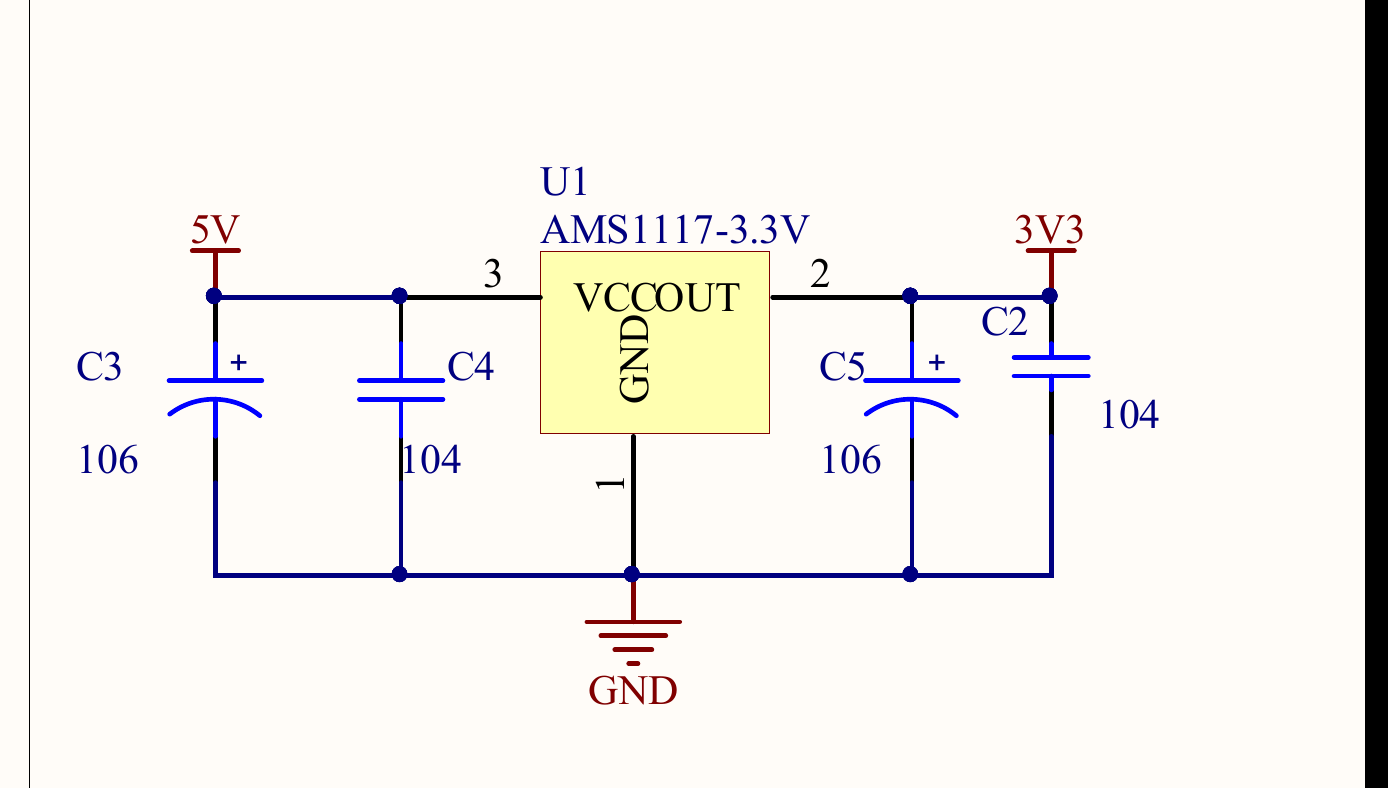
\includegraphics[width=\linewidth]{latex_assets/fig6_power.png}
\end{minipage}\hfill
\begin{minipage}[c]{0.51\linewidth}
  \centering
  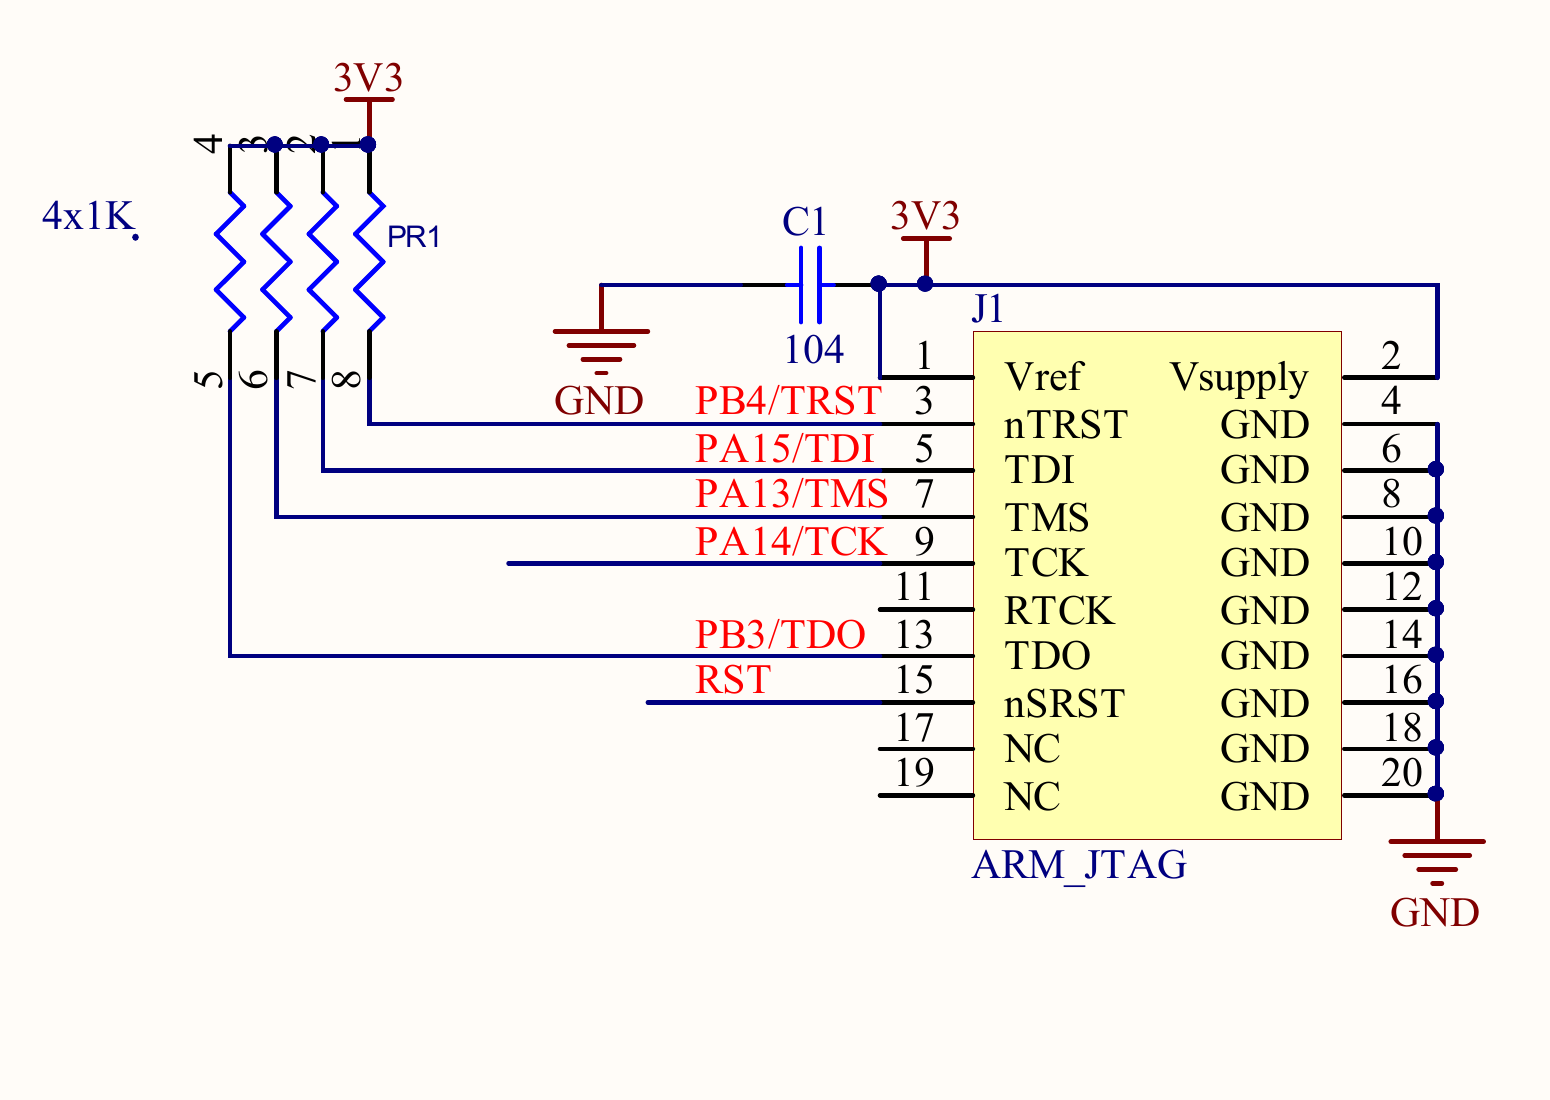
\includegraphics[width=\linewidth]{latex_assets/fig6_debug.png}
\end{minipage}
\par\vspace{9pt}
\begin{minipage}[c]{0.27\linewidth}
  \centering
  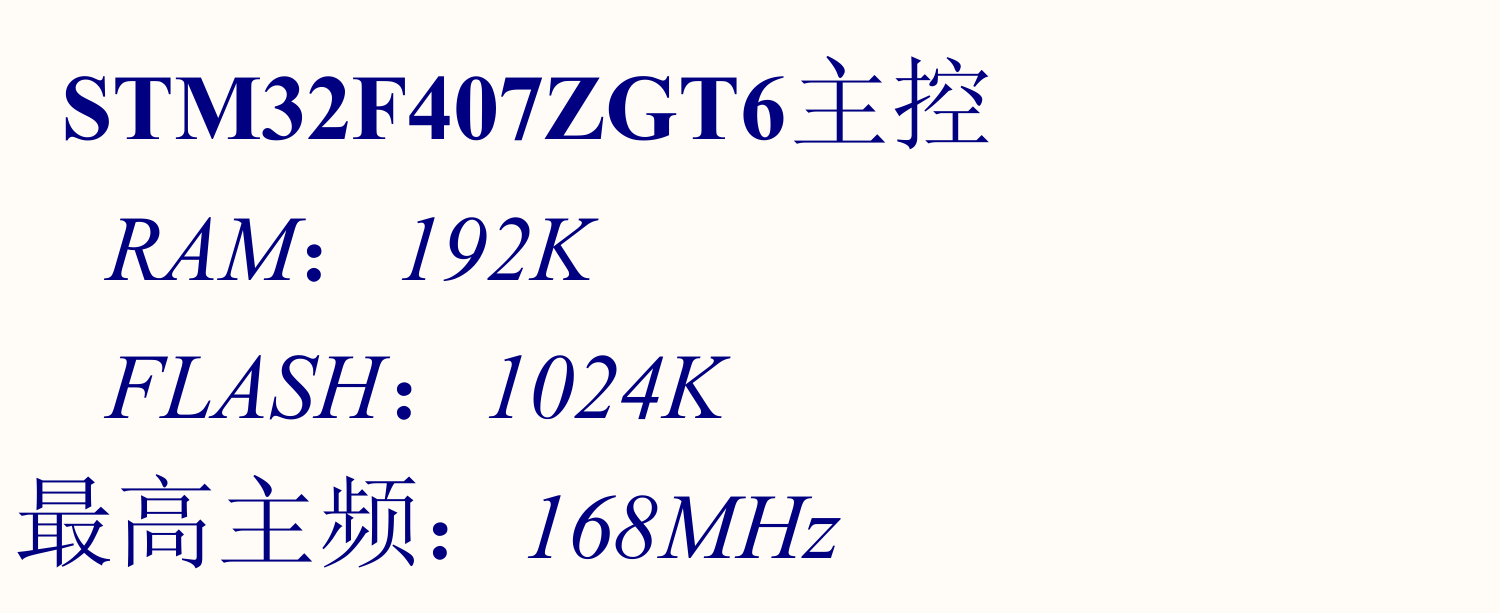
\includegraphics[width=\linewidth]{latex_assets/fig6_model.png}
  \par\vspace{16pt}
  
\includegraphics[width=\linewidth]{latex_assets/fig6_boot.png}
\end{minipage}\hfill
\begin{minipage}[c]{0.68\linewidth}
  \centering
  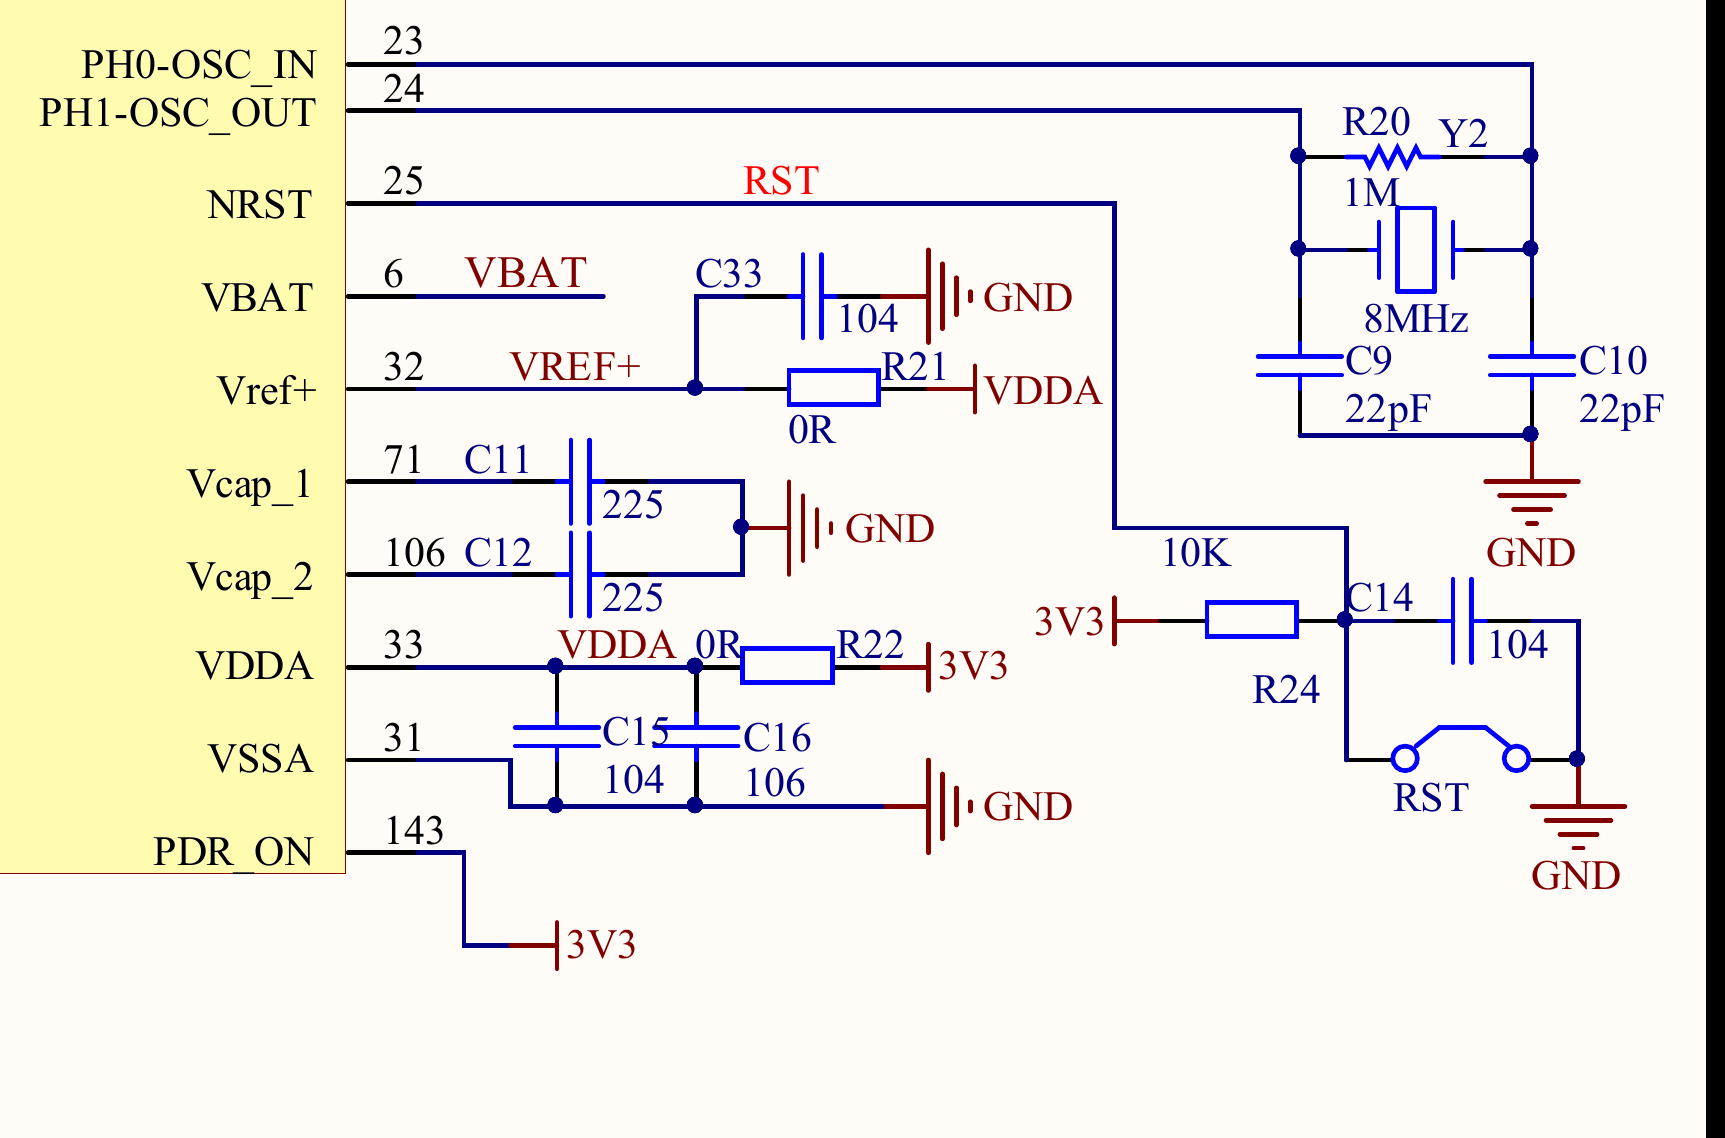
\includegraphics[width=\linewidth]{latex_assets/fig6_clock_reset.png}
\end{minipage}
\par\vspace{8pt}
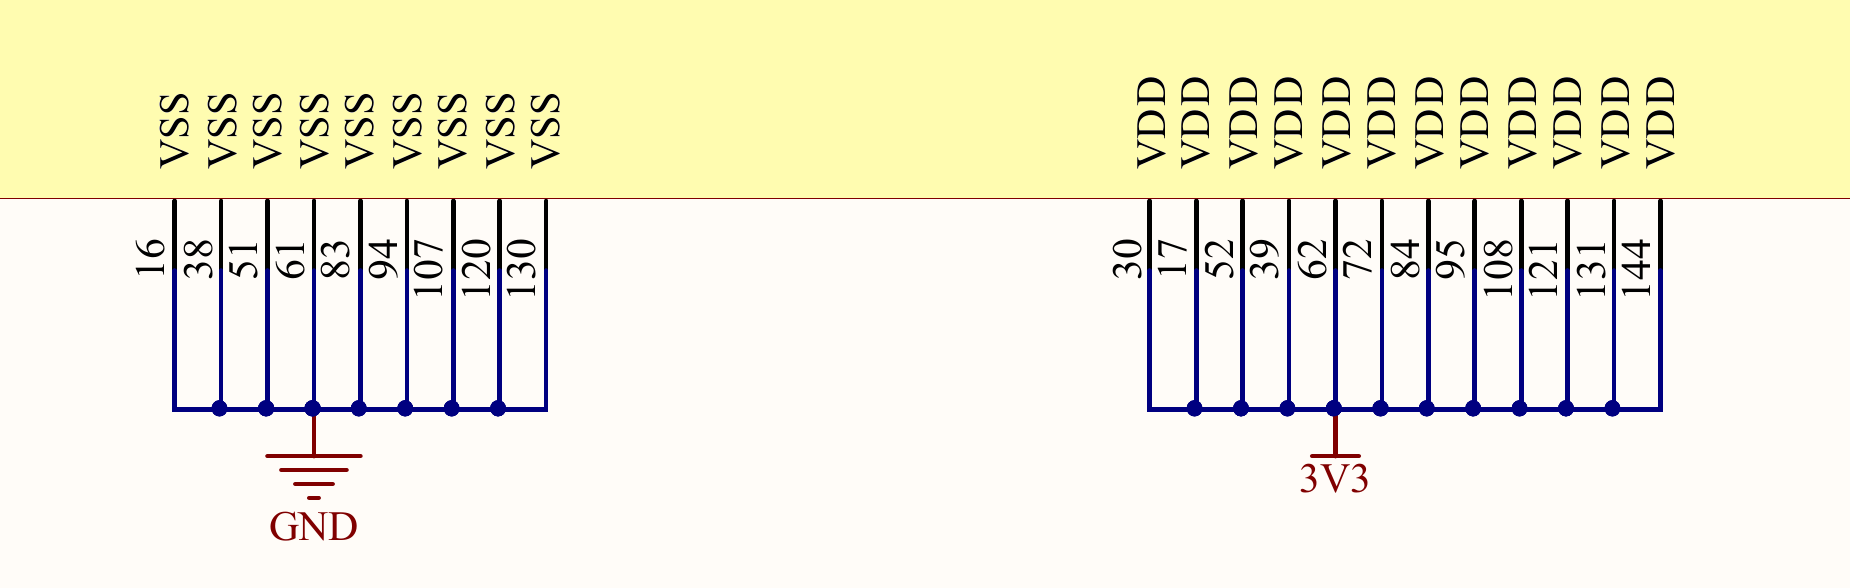
\includegraphics[width=0.94\linewidth]{latex_assets/fig6_vdd_vss.png}
\par\vspace{7pt}
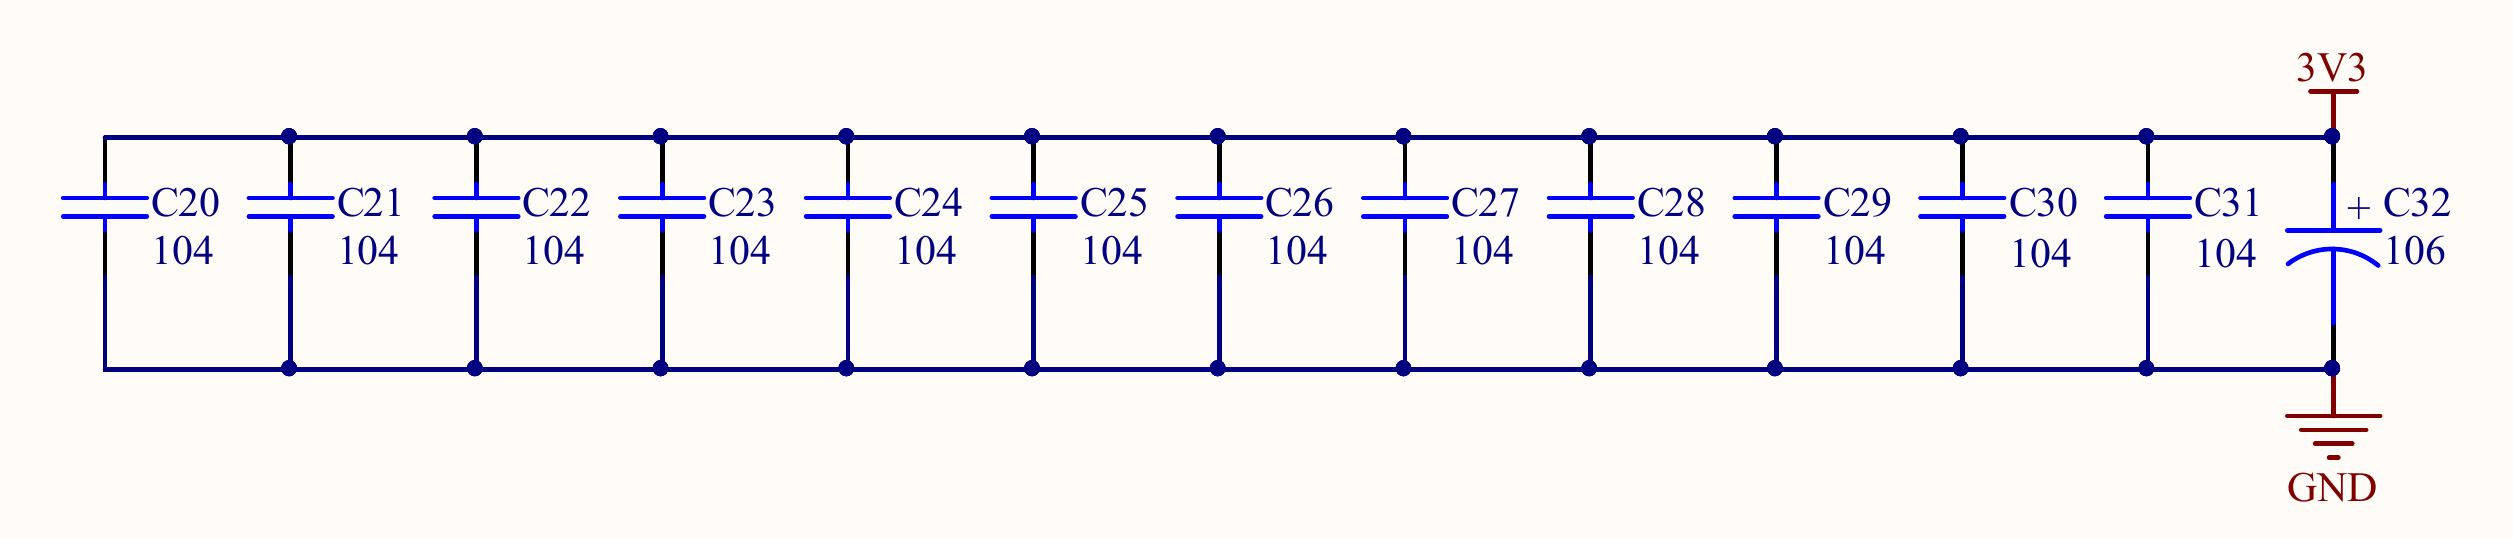
\includegraphics[width=0.94\linewidth]{latex_assets/fig6_decoupling.png}
\end{minipage}}
\caption{STM32F407ZGT6 最小系统的供电 调试 时钟 复位与启动电路}
\end{figure}

STM32F407ZGT6 最小系统涵盖主芯片工作所需的核心支撑电路：包括电源供电滤波、VCAP1/2 稳压滤波端（各外接 2.2 $\mu$F 电容）、HSE/LSE 晶振电路、NRST 按键复位、BOOT0 启动电平及 SWD 调试下载接口。同类电源与地引脚须逐一就近接入去耦电容，确保电源完整性。

\clearpage
\subsection{构建标准库与 HAL 库空白工程，理解模板的作用}

工程包括 SPL\_GPIO 和 HAL\_GPIO 两个目录，各有 Blank 空白模板与 Template GPIO 示例。Group 按功能组织源文件；\code{main.c} 是应用入口；模板统一芯片型号、头文件路径、宏定义、启动文件和链接配置。

\begin{datatab}
\captionof{table}{两类工程的组成}
\begin{tabularx}{\linewidth}{@{}C{26mm}Y Y@{}}
\toprule
\TableHead{组成} & \TableHead{标准库 SPL} & \TableHead{HAL}\\
\midrule
用户程序 & \code{main\_blank.c} 或 \code{main.c}，中断处理文件 & \code{main\_blank.c} 或 \code{main.c}，中断处理文件\\
启动文件 & \shortcell{\code{startup\_stm32f40\_41xxx.s}} & \shortcell{\code{startup\_stm32f407xx.s}}\\
内核与系统 & CMSIS、\code{system\_stm32f4xx.c} & CMSIS、\code{system\_stm32f4xx.c}\\
外设驱动 & \shortcell{STM32F4xx 标准外设驱动} & \shortcell{STM32F4xx HAL 驱动}\\
空白模板流程 & \shortcell{\code{main}\ $\to$\ \code{while (1)}} & \shortcell{\code{HAL\_Init}\ $\to$\ \code{SystemClock\_Config}\ $\to$\ \code{while (1)}}\\
\bottomrule
\end{tabularx}
\end{datatab}

\subsection{分析启动文件中的向量表、堆栈与复位序列}

本工程启动文件包含 98 个向量表项：16 个系统表项和 82 个外部中断表项，共 392 字节。\code{Stack\_Size = 0x00000400}，栈为 1 KB；\code{Heap\_Size = 0x00000200}，堆为 512 B。DCD 按 32 位字放置表项。

\begin{lstlisting}[language={},basicstyle=\linespread{1}\ttfamily\fontsize{9.2}{11.8}\selectfont,numbers=none,xleftmargin=6pt]
__Vectors       DCD     __initial_sp
                DCD     Reset_Handler
                DCD     NMI_Handler
                DCD     HardFault_Handler

Reset_Handler   PROC
                EXPORT  Reset_Handler [WEAK]
                IMPORT  SystemInit
                IMPORT  __main
                LDR     R0, =SystemInit
                BLX     R0
                LDR     R0, =__main
                BX      R0
                ENDP
\end{lstlisting}

\begin{figure}[!ht]
\centering
\begin{tikzpicture}
  \node[block,text width=2.0cm,minimum height=1.1cm] (a) at (1.1,0) {硬件装载\\MSP 与 PC};
  \node[block,text width=2.5cm,minimum height=1.1cm] (b) at (4.2,0) {\code{Reset\_Handler}};
  \node[block,text width=2.05cm,minimum height=1.1cm] (c) at (7.35,0) {\code{SystemInit}};
  \node[block,text width=2.0cm,minimum height=1.1cm] (d) at (10.2,0) {\code{\_\_main}};
  \node[block,text width=1.75cm,minimum height=1.1cm] (e) at (12.95,0) {\code{main}};
  \foreach \u/\v in {a/b,b/c,c/d,d/e}{\draw[arrow] (\u.east)--(\v.west);}
  \node[align=center,text width=4.5cm,font=\fontsize{10}{14}\selectfont] at (10.2,-1.15) {初始化数据区与零初始化区};
\end{tikzpicture}
\caption{从复位到 C 程序入口的执行顺序}
\end{figure}

从主 Flash 启动时，芯片将 Flash 映射到地址 0。处理器从 \hex{00000000} 读取初始 MSP，从 \hex{00000004} 读取复位入口。\code{SystemInit} 完成内核与系统初始化；C 运行库 \code{\_\_main} 初始化数据区后调用 \code{main}。

\clearpage
\subsection{新建 GPIO 工程，体会标准库与 HAL 库的使用}

PF9 接低电平点亮的 LED，PE4 接按下接地的按键。PF9 配置为推挽输出，PE4 配置为上拉输入；按键按下时输出低电平，LED 点亮。

\subsection*{标准库程序}
\begin{lstlisting}
#include "stm32f4xx.h"

static void GPIO_Setup(void)
{
    GPIO_InitTypeDef gpio;
    RCC_AHB1PeriphClockCmd(
        RCC_AHB1Periph_GPIOF | RCC_AHB1Periph_GPIOE, ENABLE);

    GPIO_SetBits(GPIOF, GPIO_Pin_9);
    GPIO_StructInit(&gpio);
    gpio.GPIO_Pin = GPIO_Pin_9;
    gpio.GPIO_Mode = GPIO_Mode_OUT;
    gpio.GPIO_OType = GPIO_OType_PP;
    gpio.GPIO_Speed = GPIO_Speed_2MHz;
    gpio.GPIO_PuPd = GPIO_PuPd_NOPULL;
    GPIO_Init(GPIOF, &gpio);

    gpio.GPIO_Pin = GPIO_Pin_4;
    gpio.GPIO_Mode = GPIO_Mode_IN;
    gpio.GPIO_PuPd = GPIO_PuPd_UP;
    GPIO_Init(GPIOE, &gpio);
}

int main(void)
{
    GPIO_Setup();
    while (1)
    {
        if (GPIO_ReadInputDataBit(GPIOE, GPIO_Pin_4) == Bit_RESET)
            GPIO_ResetBits(GPIOF, GPIO_Pin_9);
        else
            GPIO_SetBits(GPIOF, GPIO_Pin_9);
    }
}
\end{lstlisting}

\begin{datatab}
\captionof{table}{按键输入与 LED 输出关系}
\begin{tabularx}{\linewidth}{@{}C{28mm}C{34mm}C{34mm}Z@{}}
\toprule
\TableHead{按键状态} & \TableHead{PE4 输入} & \TableHead{PF9 输出} & \TableHead{LED 状态}\\
\midrule
松开 & 高电平 & 高电平 & 熄灭\\
按下 & 低电平 & 低电平 & 点亮\\
\bottomrule
\end{tabularx}
\end{datatab}

\clearpage
\subsection*{HAL 初始化与主循环}
\begin{lstlisting}
#include "main.h"

static void SystemClock_Config(void);
static void GPIO_Setup(void);

int main(void)
{
    HAL_Init();
    SystemClock_Config();
    GPIO_Setup();
    while (1)
    {
        GPIO_PinState key = HAL_GPIO_ReadPin(GPIOE, GPIO_PIN_4);
        HAL_GPIO_WritePin(GPIOF, GPIO_PIN_9, key);
    }
}

static void GPIO_Setup(void)
{
    GPIO_InitTypeDef gpio = {0};
    __HAL_RCC_GPIOF_CLK_ENABLE();
    __HAL_RCC_GPIOE_CLK_ENABLE();

    HAL_GPIO_WritePin(GPIOF, GPIO_PIN_9, GPIO_PIN_SET);
    gpio.Pin = GPIO_PIN_9;
    gpio.Mode = GPIO_MODE_OUTPUT_PP;
    gpio.Pull = GPIO_NOPULL;
    gpio.Speed = GPIO_SPEED_FREQ_LOW;
    HAL_GPIO_Init(GPIOF, &gpio);

    gpio.Pin = GPIO_PIN_4;
    gpio.Mode = GPIO_MODE_INPUT;
    gpio.Pull = GPIO_PULLUP;
    HAL_GPIO_Init(GPIOE, &gpio);
}
\end{lstlisting}

\begin{datatab}
\captionof{table}{标准库与 HAL 的 GPIO 函数}
\begin{tabularx}{\linewidth}{@{}C{19mm}Z Z@{}}
\toprule
\TableHead{操作} & \TableHead{标准库 SPL} & \TableHead{HAL}\\
\midrule
使能时钟 & \code{RCC\_AHB1PeriphClockCmd} & \code{\_\_HAL\_RCC\_GPIOx\_CLK\_ENABLE}\\
初始化 & \code{GPIO\_Init} & \code{HAL\_GPIO\_Init}\\
读取引脚 & \code{GPIO\_ReadInputDataBit} & \code{HAL\_GPIO\_ReadPin}\\
写入引脚 & \code{GPIO\_SetBits / GPIO\_ResetBits} & \code{HAL\_GPIO\_WritePin}\\
\bottomrule
\end{tabularx}
\end{datatab}

在底层硬件机制上：读引脚函数通过输入数据寄存器（IDR）获取引脚物理电平；写引脚函数则借助端口置位/复位寄存器（BSRR）实现原子操作。BSRR 属于只写命令寄存器（读操作恒返回 0），低 16 位写 1 置高，高 16 位写 1 置低，写 0 保持不变，单次 32 位总线写操作即可完成电平翻转，规避了对输出数据寄存器 ODR 执行读-改-写（\code{|=} 或 \code{\&=}）可能引发的中断竞态风险。此外，配置结构体中的输出速度控制的是推挽 MOS 管的压摆率（Slew Rate），用于抑制高频辐射干扰，其物理特性独立于软件逻辑翻转频率。

\end{document}
